\documentclass[tikz,border=2pt]{standalone}
\usepackage[utf8]{inputenc}
\usepackage{tikz}
\usepackage{pgfplots}
\usetikzlibrary{positioning}

% \title{empirical_cdf_tikz}
% \author{Vishal Ghoniya}
% \date{July 2022}

\pgfplotsset{compat=1.18}
\begin{document}

% \maketitle
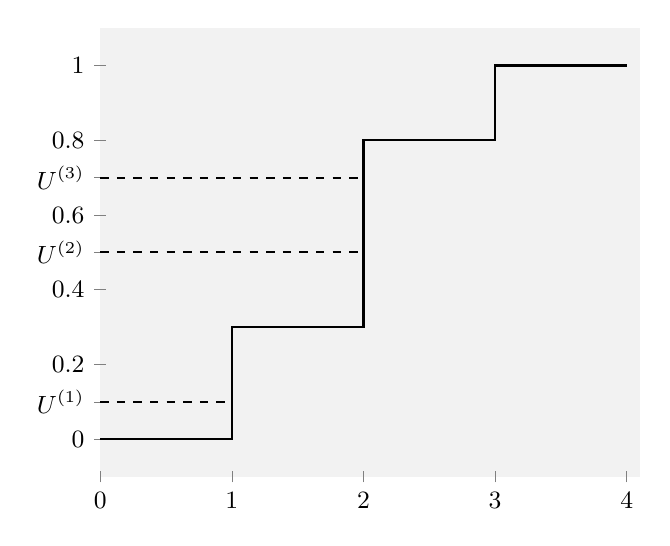
\begin{tikzpicture}[font={\small}]
\begin{axis}[axis line style={opacity=0}, 
    axis lines=left, ytick={0.0,0.2,...,1.0},
    ymax=1.1, ymin=-0.1, 
    xtick={0,1,...,4}, 
    xmax=4.1, 
    axis background/.style={fill=gray!10}, 
    extra y ticks={0.1,0.5,0.7},
    extra y tick labels={{$U^{(1)}$},{$U^{(2)}$},{$U^{(3)}$}}]
\addplot+[const plot, no marks, thick, black] coordinates {(0,0) (1,0.3) (2,0.3) (2,0.8) (3,0.8) (3,0.8) (3,1) (4,1)};
\addplot+[const plot, no marks, dashed, thick, black] coordinates {(0,0.1) (1,0.1)};
\addplot+[const plot, no marks, dashed, thick, black] coordinates {(0,0.7) (2,0.7)};
\addplot+[const plot, no marks, dashed, thick, black] coordinates {(0,0.5) (2,0.5)};
\end{axis}

\end{tikzpicture}
\end{document}
